\subsection{Modeling}
\label{4c_modeling}

	The model for the \textit{PDSurvey} platform is maintained with the help of the Node package Mongoose. Node.js maps the route parameters and routes all requests to the corresponding Mongoose model. Angular.js builds its model upon the REST API and maps it via dynamic two-way-binding to it's scope. Thus all changes to the model originate from Mongoose.



\subsubsection{Development Process / Modeling}

	The development process of the PDSurvey platform was inspired and influenced by the following approaches:

	\begin{itemize}
	\item working agile and user centered... TODO: look up how to best explain it.

	\item User Centered Design: (paper nr 31): ``constitutes an iterative process of system design, deployment and evaluation'' (quote from paper 31). Work iteratively, continuous deployment and evaluation.

	\item Concept of extreme programming\footnote{\url{http://www.extremeprogramming.org/rules.html} (accessed on November 14, 2014)}: First user stories were written and assessed in a small group. The next step was to transfer these stories to user models, describing in detail which functionality the stakeholders of PDSurvey are supposed to have. Later a first software architecture and software model was built, getting more specific. Dependencies between models were defined and this model was continuously refined and improved throughout the dvelopment phase. The last step of the modeling represented screen designs, getting a clear view of what the interface might later look like.

	\item Used the extreme programming\footnote{\url{http://www.extremeprogramming.org/rules.html} (accessed on November 13, 2014)} approach: user stories, release planning, release schedule, small releases, iterating


	\item criteria for good user stories: http://tigertechtalk.wordpress.com/2012/10/17/wie-schreibe-ich-eine-gute-user-story-und-was-ist-das-uberhaupt/
	\end{itemize}








\subsubsection{User roles}

As of now only two roles are implemented, the admin-role and the guest-role.

% FEEDBACK VON FLORIAN: nein, nicht zu komplex machen. Es sollte sogar reichen, nur zwischen Admin & Operator (= Application Provider) zu unterscheiden, da der end user (das Public Display) ja sowieso nur auf die öffentlichen REST API Zugriff hat. (2014-11-14)


In the long term it would be desirable to have the following user roles: Admin, Operator, Evaluator, DisplayApplication.






\subsubsection{Software model}

In total there are the following classes.

\begin{enumerate}
\item list all classes
\item 1 UML diagram is enough, according to Florian
\end{enumerate}


\subsubsection{Dependencies}

Of special interest are the following four models: Survey, Display, Campaign and Responses.

\paragraph{Surveys:} Surveys resembles the foundation of PDSurvey, with the aim of reuse and standardization. A survey consists of multiple sections, being built of of multiple questions. Each question is of a corresponding question type and every survey belongs to a category. This allows the filtering for relevant surveys. To be able to create private surveys, not being shared across the entire platform, every survey is assigned to an individual user.

\paragraph{Displays:} In the display collection all displays connected to the PDSurvey platform are contained. To allow for an evaluation across multiple display models and based on the context of the displays, the display model and a static and/or dynamic context is assigned to every display.

\paragraph{Campaigns:} Campaigns resemble the most integral part, since they glue all of the pieces together and allow the distribution of surveys to public display networks. A campaign consists of displays and surveys and creates the mapping of the questionnaires to public displays. Additionally to each of those mapping an individual context can be assigned, enabling the later comparison of results in between the public displays.

\paragraph{Responses:} All responses made to each survey are logged in the Response collection. The queries are carried out individually per user, per display and per campaign. This model will be the base for further extensions, amongst others the automatic evaluation of the survey responses and the comparison inbetween an entire display network, to be able to find out which properties of a display might be related to certain effects.

\paragraph{Context:} One of the benefits of creating such a survey platform is being able to collect and evaluate large amounts of data, without having to pay more people for conducting and evaluating the survey. The idea would be to collect a large number of responses from a variety of displays in various settings, and assigning a specific context to every display connected to PDSurvey. Once enough data is collected, having the ability to evaluate and compare the displays between each other. Interesting questions for analysis would be, which role the context plays on how the users behave, when running identical software settings on the displays, but only varying the context (position, size of display, surrounding environment of the display, positioning it outdoors or indoors, influence of the weather, type of building it is positioned in).


\begin{figure}%[btph]
    \begin{center}
        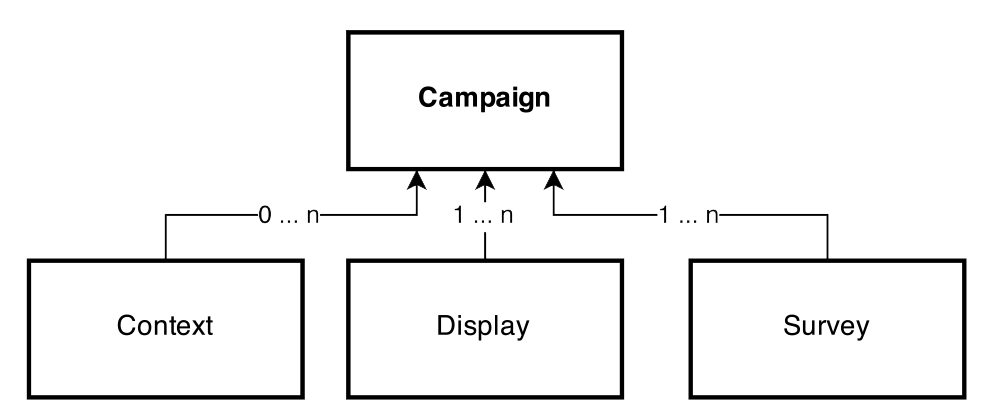
\includegraphics[width=.8\columnwidth]{img/4_implementation/4-dependency-campaign}
    \end{center}
 % \begin{center}\LARGE [BILD]\end{center}
 \caption{Campaign model dependencies}
 \label{fig:4-dependency-campaign}
\end{figure}


++ neue Namensgebung, um in der domain specific language zu bleiben --> application provider / display provider / space provider (anstatt Operator). Wir werden aber nur mit dem Application Provider (anstatt Operator) im System arbeiten





\subsubsection{REST interface}

Defining the REST API. 

% TODO: Explain why I chose which level of separation / detail.

Notes from before I started writing
\begin{enumerate}
\item Think about using a Extreme Programming approach http://www.extremeprogramming.org/rules.html
\end{enumerate}